\documentclass[tikz,border=2pt,11pt]{standalone}
\usepackage{amsmath}
\usepackage{amssymb}
\usepackage{tikz}
\newcommand{\E}{\mathbb E}
\newcommand{\Pp}{\mathbb P}
\newcommand{\one}{\mathbf1}
\DeclareMathOperator{\diam}{diam}
\DeclareMathOperator{\Var}{Var}
\newcommand{\Prob}{\mathbb P}
\newcommand{\ind}{\mathbf1}
\newcommand{\R}{\mathbb R}
\newcommand{\N}{\mathbb N}
\newcommand{\Z}{\mathbb Z}
\begin{document}
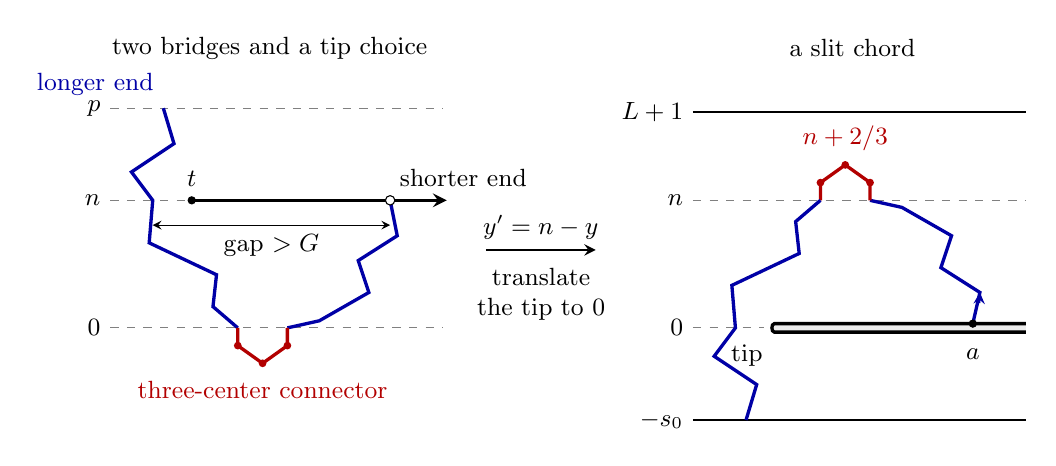
\begin{tikzpicture}[x=.9cm,y=.9cm,>=stealth,font=\small]
  \begin{scope}
    \node[align=center] at (1.1,3.95) {two bridges and a tip choice};
    \foreach \y/\lab in {0/{0},1.8/{n},3.1/{p}}
      {\draw[dashed,gray] (-1.15,\y)--(3.55,\y);
       \node[left] at (-1.15,\y) {$\lab$};}
    \draw[very thick,blue!65!black] (.65,0)--(.3,.3)--(.35,.75)
      --(-.6,1.2)--(-.55,1.8)--(-.85,2.2)--(-.25,2.6)--(-.4,3.1);
    \draw[very thick,blue!65!black] (1.35,0)--(1.8,.1)--(2.5,.5)
      --(2.35,.95)--(2.9,1.3)--(2.8,1.8);
    \draw[very thick,red!70!black] (.65,0)--(.65,-.25)
      --(1,-.5)--(1.35,-.25)--(1.35,0);
    \foreach \x/\y in {.65/-.25,1/-.5,1.35/-.25}
      {\fill[red!70!black] (\x,\y) circle (1.4pt);}
    \draw[very thick,->] (0,1.8)--(3.6,1.8);
    \fill (0,1.8) circle (1.5pt);
    \draw[fill=white] (2.8,1.8) circle (1.7pt);
    \node[above] at (0,1.86) {$t$};
    \node[above right] at (2.8,1.86) {shorter end};
    \node[below,red!70!black] at (1,-.62) {three-center connector};
    \draw[<->] (-.55,1.45)--(2.8,1.45)
      node[midway,below] {gap $>G$};
    \node[above left,blue!65!black] at (-.4,3.15) {longer end};
  \end{scope}
  \draw[->,thick] (4.15,1.1)--(5.7,1.1)
    node[midway,above,align=center] {$y'=n-y$};
  \node[below,align=center] at (4.93,.98) {translate\\the tip to $0$};
  \begin{scope}[xshift=7.4cm]
    \node[align=center] at (1.1,3.95) {a slit chord};
    \draw[thick] (-1.15,3.05)--(3.55,3.05);
    \draw[thick] (-1.15,-1.3)--(3.55,-1.3);
    \node[left] at (-1.15,3.05) {$L+1$};
    \node[left] at (-1.15,-1.3) {$-s_0$};
    \draw[dashed,gray] (-1.15,1.8)--(3.55,1.8);
    \node[left] at (-1.15,1.8) {$n$};
    \draw[dashed,gray] (-1.15,0)--(-.14,0);
    \node[left] at (-1.15,0) {$0$};
    \fill[gray!15] (0,.06)--(3.55,.06)--(3.55,-.06)--(0,-.06)
      to[out=180,in=180] (0,.06);
    \draw[very thick] (3.55,.06)--(0,.06)
      to[out=180,in=180] (0,-.06)--(3.55,-.06);
    \draw[very thick,blue!65!black] (2.8,.06)--(2.9,.5)--(2.35,.85)
      --(2.5,1.3)--(1.8,1.7)--(1.35,1.8);
    \draw[very thick,red!70!black] (1.35,1.8)--(1.35,2.05)
      --(1,2.3)--(.65,2.05)--(.65,1.8);
    \foreach \x/\y in {.65/2.05,1/2.3,1.35/2.05}
      {\fill[red!70!black] (\x,\y) circle (1.4pt);}
    \draw[very thick,blue!65!black] (.65,1.8)--(.3,1.5)--(.35,1.05)
      --(-.6,.6)--(-.55,0)--(-.85,-.4)--(-.25,-.8)--(-.4,-1.3);
    \fill (2.8,.06) circle (1.5pt);
    \draw[->,blue!65!black,thick] (2.89,.35)--(2.9,.5);
    \node[below] at (2.8,-.16) {$a$};
    \node[above,red!70!black] at (1,2.36) {$n+2/3$};
    \node[below left] at (-.03,-.1) {tip};
  \end{scope}
\end{tikzpicture}
\end{document}
